% !TEX root = ../thesis.tex
\section{Parametrizace řečového signálu}
\label{chap:asr:parametrization}

Stejně jako v~mnoha jiných odvětvích, i při rozpoznávání řeči je inspirací člověk. Pro získání sekvence pozorování (příznaků) vycházíme z \textbf{modelování produkce řeči} a \textbf{modelování procesu slyšení}.

\subsection{Modelování produkce řeči}
\label{chap:asr:parametrization:production}

Cílem modelování produkce řeči je nalezení matematických vztahů, které poslouží k~reprezentaci fyzikálních dějů spojených s~produkcí řeči. Základem je parametrizační technika \textbf{lineárního prediktivního kódování}, známá pod anglickou zkratkou LPC\footnote{Linear Predictive Coding} \cite{Benesty2007}. Vychází z představy, že hlasové ústrojí člověka je schopno vytvářet tři různé typy řečových zvuků:

\begin{itemize}
  \item \textit{samohlásky} - ty se řadí mezi znělé typy zvuků produkované periodickým buzením vznikajícím pulsy vzduchu, které jsou produkovány hlasivkami;
  \item \textit{frikativy} (např. $/f/$\footnote{Zápis $/f/$ symbolizuje foném, což je akustická reprezentace písmene, \textit{f}. Konkrétní zápisy se mohou lišit podle použité fonetické abecedy. V~Čechách se nejčastěji používá abeceda $SAMPA$ či $Z\check{C}FA$.}) - někdy nazývané jako třené souhlásky, protože vznikají třením vydechovaného proudu vzduchu o překážku, kterou mouhou být například zuby nebo jazyk, v~některém místě hlasového ústrojí;
  \item \textit{explozivy} (např. $/b/$, $/p/$ ap.) - také nazývané jako souhlásky výbuchové, se tvoří úplným uzavřením vydechovaného proudu vzduchu pomocí artikulačních orgánů. To se následně projeví jako krátká pauza (tzv. okluze), po které následuje náhlé jednorázové uvolnění a únik nahromaděného vzduchu (tzv. exploze) \cite{Psutka2006}.
\end{itemize}

% Snahou je navrhnout takový model hlasového traktu, který bude dobře popisovat výše zmíněné řečové zvuky. Nesmí se však zapomenout na možnou přílišnou složitost~a nedostatečnou přesnost modelu. Jako ideální se může jevit lineárně časově invariantní model.
Bohužel lidskou řeč lze klasifikovat jako kontinuální časově variantní a v~některých situacích dokonce nelineární proces, proto je téměř nemožné jej přesně namodelovat. Pokud však budeme předpokládat, že v~konkrétním krátkém časovém úseku zůstává buzení a parametry hlasivkového traktu přibližně konstantní, tak je možné navrhnout lineární časově invariantní model řeči, který je platný pro krátké časové úseky.
% Tuto podmínku lze považovat za platnou
Pro intervaly o délce od $10$ do $30\ ms$ lze považovat podmínku za platnou.
% Odtud také vychází uvažovaná perioda segmentů řeči, zmíněná v~úvodu této kapitoly.
Pro tyto segmenty je možné proces vytváření řeči modelovat pomocí tzv. \textbf{krátkodobého modelu}, který má v~krátkých časových intervalech pevné parametry \cite{Holmes2001}.

% Odvození obecného diskrétního modelu hlasivkového traktu je založeno na zjednodušeném modelu produkce řeči, jehož struktura je ukázána na obr. \ref{fig:asr:model:speech}. Ten je tvořen třemi dílčími částmi, konkrétně modelem hlasivek, modelem hlasivkového traktu a modelem vyzařovaného zvuku. K odvození a popisu vlastností modelu se využívá výhod Z-transformace \cite{Psutka2006}.

% \begin{figure}[hbpt]
%   \centering
%   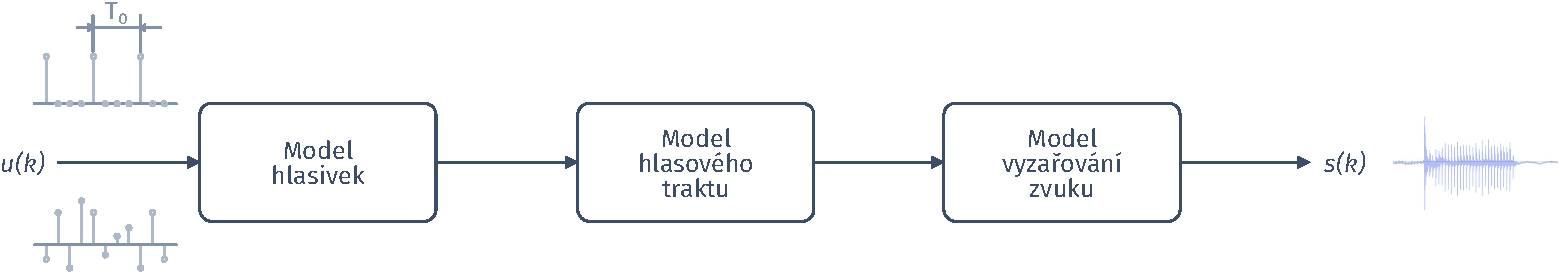
\includegraphics[width=0.9\textwidth]{./ch4-asr/img/speech_model.pdf}
%   \caption{Blokové schéma modelu produkce řeči.}
%   \label{fig:asr:model:speech}
% \end{figure}

% Krátkodobý model produkce řeči lze aproximovat celopólovým modelem charakteru filtru $H(z)$ ve tvaru

% \begin{equation}
%   H(z) = \frac{G}{1 + \sum_{i = 1}^{Q} a_{i} z^{-i}} = \frac{G}{A(z)},
%   \label{eq:asr:lpc:generic}
% \end{equation}

% \noindent kde $G$ představuje celkové zesílení, $Q$ je řád modelu a $a_i$ jsou parametry modelu. Vstupem modelu je buzení $u(k)$ (viz obr. \ref{fig:asr:model:speech}), které je v~případě znělých zvuků reprezentováno sledem pulsů s~periodou $T_0$\footnote{Perioda základního hlasivkového tónu.} a pro neznělé zvuky je tvořeno náhodným šumem s~plochým spektrem. V~časové oblasti je pak diskrétní výstupní odezva při fixovaných parametrech hlasového traktu ($10 - 30\ ms$) dána konvolucí buzení a impulzní odezvy krátkodobého modelu. Na základě toho je možné model upravit do podoby znázorněné na obr. \ref{fig:asr:model:speech:excitation}, kde $u(k)$ je buzení a $s(k)$ je výstupní signál s~parametry hlasového ústrojí odpovídajícími parametrům $a_i$ celopólového modelu.

% \begin{figure}[hbpt]
%   \centering
%   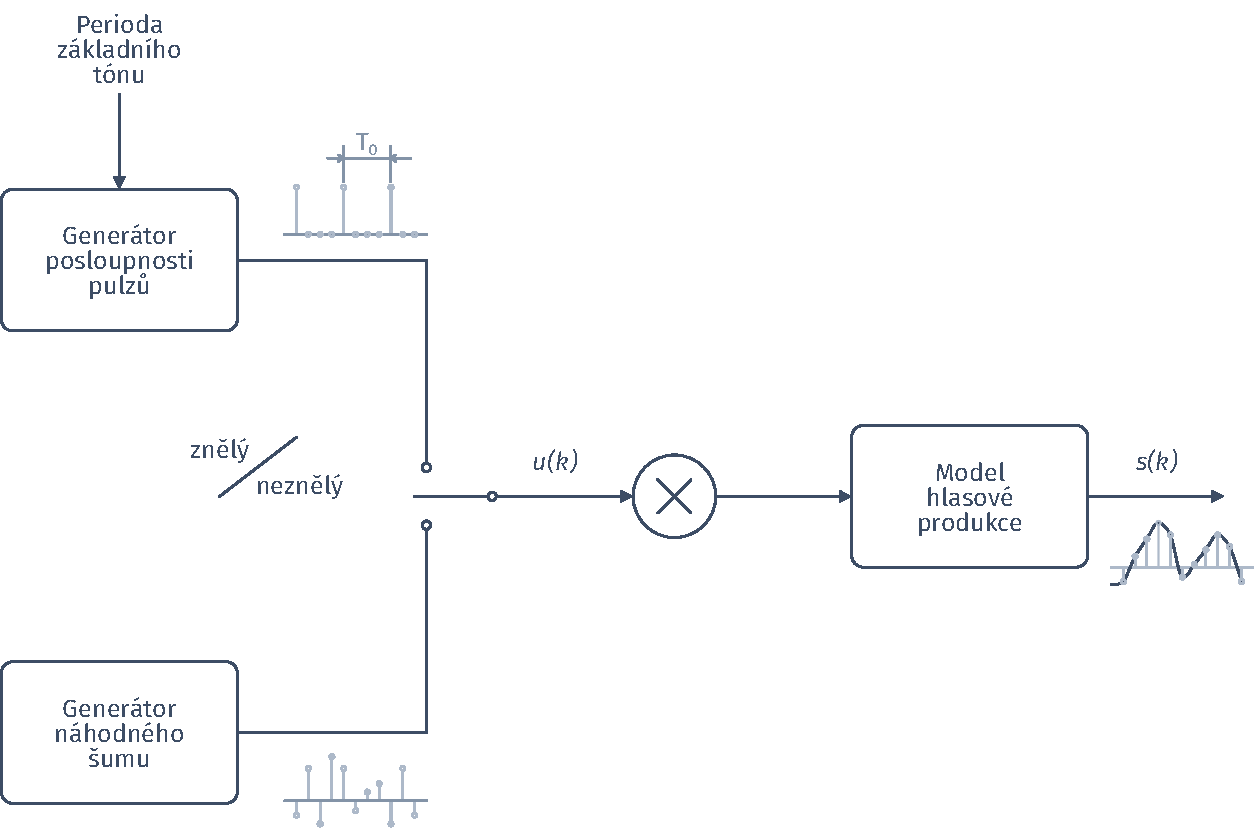
\includegraphics[width=0.9\textwidth]{./ch4-asr/img/speech_process.pdf}
%   \caption{Blokové schéma upraveného modelu produkce řeči.}
%   \label{fig:asr:model:speech:excitation}
% \end{figure}

% K odhadu parametrů $a_i$ slouží \textbf{lineární prediktivní analýza}. Odhad probíhá přímo z krátkodobého řečového signálu. Přenosové vlastnosti krátkodobého modelu je možné popsat rovnicí (\ref{eq:asr:lpc:generic}). Myšlenka metody LPC vychází z předpokladu, že vzorek $k$ řečového signálu je možné popsat lineární kombinací $Q$ předchozích vzorků a buzení $u(k)$, což lze matematicky vyjádřit pomocí následující rovnice ve tvaru

% \begin{equation}
%   s(k) = - \sum_{i = 1}^{Q} a_i s(k-1) + Gu(k).
%   \label{eq:asr:lpc:generic:edited}
% \end{equation}

% \noindent %Z rovnice (\ref{eq:asr:lpc:generic:edited})
% Je patrné, že se LPC snaží odhadnout parametry modelu $a_i$ a zesílení $G$ pomocí známé reálně naměřené posloupnosti vzorků řeči $s(k)$. K odhadu se používá principu minimalizace kvadratické chyby krátkodobé energie signálu $e\left(k\right)$. Ta je v~časové oblasti popsána vztahem

% \begin{equation}
%   E = \sum_{k} e^2(k) = \sum_{k} \left[ s(k) - s'(k)\right]^2 = \sum_{k} \left( s(k) + \sum_{i = 1}^{Q} a_i s(k-1) + Gu(k) \right),
% \end{equation}

% \noindent kde $s(k)$ jsou vzorky reálného řečového signálu a $s'(k)$ jsou ty predikované LPC filtrem. Pro nalezení minimální hodnoty krátkodobé chyby predikce $E$ pro konkrétní analyzovaný segment, je použita metoda nejmenších čtverců. K výpočtu konkrétních koeficientů modelu $a_i$ je možné použít rekurzivního Durbinova algoritmu \cite{Holmes2001}.

% Další zpřesnění popisu hlasového traktu lze provést pomocí \textbf{kepstrálních koeficientů lineární predikce} $c\left(k\right)$. Kepstrum k-tého mikrosegmentu řečového signálu $s\left(k\right)$ je definováno vztahem % (\ref{eq:asr:lpc:cepstrum:generic}),

% \begin{equation}
%   c(k) = \mathcal{F}^{-1}\left\{\log\left| \mathcal{F}\left\{s(k)\right\} \right|\right\}.
%   \label{eq:asr:lpc:cepstrum:generic}
% \end{equation}

% \noindent kde $\mathcal{F}$ představuje operátor diskrétní Fourierovy transformace (DFT) a $\mathcal{F}^{-1}$ reprezentuje inverzní diskrétní Fourierovu transformaci (IDFT). Postup výpočtu je znázorněn na obr. \ref{fig:asr:model:speech:cepstrum}.

% \begin{figure}[hbpt]
%   \centering
%   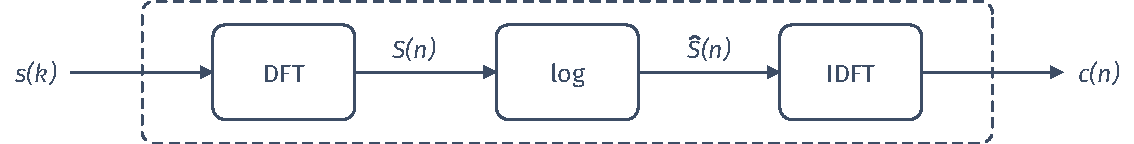
\includegraphics[width=0.9\textwidth]{./ch4-asr/img/cepstrum.pdf}
%   \caption{Blokové schéma principu výpočtu kepstra.}
%   \label{fig:asr:model:speech:cepstrum}
% \end{figure}

% Pro získání kepstrálních koeficientů lineární predikce lze využít vztah (\ref{eq:asr:lpc:generic}), který po zlogaritmování přejde do tvaru

% \begin{equation}
%   \log H(z) = \log \left( \frac{G}{A(z)} \right).
%   \label{eq:asr:lpc:cepstrum}
% \end{equation}

% \noindent Člen $A(z)$ je polynomem proměnné $z^{-1}$ řádu $Q$. Pokud všechny jeho kořeny leží uvnitř jednotkové kružnice, tak lze aplikovat Taylorův rozvoj a vztah (\ref{eq:asr:lpc:cepstrum}) lze zapsat jako

% \begin{equation}
%   \log \left( \frac{G}{A(z)} \right) = c(0) + c(1)z^{-1} + \dots = \sum_{k=0}^{\infty} c(k)z^{-k},
%   \label{eq:asr:lpc:cepstrum:taylor}
% \end{equation}

% \noindent kde $c(k)$ jsou tzv. kepstrální koeficienty LPC. Po zderivování obou stran rovnice přejde vztah (\ref{eq:asr:lpc:cepstrum:taylor}) do tvaru

% \begin{equation}
%   - \sum_{i=1}^{Q} ia_iz^{-i} = \left( \sum_{k=0}^{\infty} kc(k)z^{-k} \right)\left( \sum_{i=0}^{Q} a_iz^{-i}\right).
%   \label{eq:asr:lpc:cepstrum:deriv}
% \end{equation}

% \noindent Jestliže se $a_i = 1$, pak lze po roznásobení pravé strany rovnice (\ref{eq:asr:lpc:cepstrum:deriv}) a po následném porovnání členů u stejných mocnin proměnné $z$ zapsat vztahy pro výpočet kepstrálních koeficientů LPC ve tvaru

% \begin{align}
%   \begin{split}
%     c(1) &= -a_1, \\
%     c(k) &=
%     \begin{cases}
%       - a_k - \sum_{i=1}^{k-1} \left(\frac{i}{k}\right) c(i) a_{k-1},  & \quad \text{pro } 2 \leq  k~\leq Q, \\
%       - \sum_{i=1}^{Q} \left(\frac{k - i}{k}\right) c(k-i) a_i,  & \quad \text{pro }  k~= Q + 1, Q + 2, \dots \quad ,
%     \end{cases}
%   \end{split}
%   \label{eq:asr:lpc:cepstrum:coef}
% \end{align}

% \noindent kde $k = 1, 2, \dots , Q^{*}$. $Q^{*}$ je počet kepstrálních koeficientů, pro které musí platit $Q^{*} \geq Q$. Kepstrální koeficienty LPC jsou vztaženy ke spektrální obálce mikrosegmentu řeči odvozené LPC analýzou.

% Spektrální obálku je následně možné získat z rovnice (\ref{eq:asr:lpc:generic}) dosazením $z = e^{j\omega}$. Pro uspokojivou reprezentaci se tradičně volí $Q$ v~rozmezí $7-15$ v~závislosti na spektrální šířce přenášeného pásma a požadované přesnosti aproximace. Z toho plyne, že pro popis mikrosegmentu řeči by mohl být dostačující příznakový vektor o~$15$ koeficientech.

\subsection{Modelování procesu slyšení}
\label{chap:asr:parametrization:hearing}

Zvuk představuje mechanické vlnění hmotných částic, které se šíří v~plynném, kapaném nebo tuhém prostředí.
Z fyziologického pohledu je však zvuk považován pouze za slyšitelné vlnění.
To je takové, které je schopno vnímat sluchové ústrojí člověka. Zpravidla se jedná o frekvence $16\ Hz - 20\ kHz$.
% Pro každého člověka je ale toto rozmezí individuální a mění se s~věkem.
% S přibývajícím věkem a sluchovou zátěží klesá hlavně horní mezní kmitočet \cite{Psutka2006}.

% To, zda je člověk schopen daný zvuk slyšet, však není závislé pouze na frekvenci zvuku.
Velmi podstatná je i intenzita zvuku, která se rovná energii zvukového vlnění procházející za jednotku času jednotkovou plochou kolmou ke směru šíření vln. Zároveň je úměrná akustickému tlaku zvukové vlny, tj. tlaku, kterým zvukové vlny působí na nějakou překážku.
% V~případě člověka lze překážkou chápat ušní bubínek.
Závislost mezi intenzitou zvuku $I\ \left[Wm^{-2}\right]$ a akustickým tlakem $p\ \left[Pa\right]$ je vyjádřen vztahem

\begin{equation}
  I = \frac{p^{2}}{z},
  \label{eq:asr:mfcc:intesity}
\end{equation}

\noindent kde $z$ je měrná akustická impedance prostředí, kterým se zvuk šíří.
% Lidské ucho je schopno vnímat akustický tlak v~rozsahu od $2\cdot10^{-5}$ až $2\cdot10^{2}\ Pa$, tj. v~rozsahu sedmi řádů. Z praktického důvodu se tedy používá logaritmické stupnice. K vyjadřování pak slouží logaritmus poměru uvažované veličiny a mezinárodně normované referenční hodnoty téže veličiny \cite{Psutka2006}. Hladina intenzity $L_{I}$ je pak definována vztahem

% \begin{equation}
%   L_{I} = 10\log_{10}\frac{I}{I_{0}},
%   \label{eq:asr:mfcc:intesity:level}
% \end{equation}

% \noindent kde $I$ představuje intenzitu zvuku a $I_{0} = 10^{-12}\ Wm^{-2}$ referenční hodnotu intenzity. Pro hladinu akustického tlaku platí

% \begin{equation}
%   L_{p} = 20\log_{10}\frac{p}{p_{0}},
%   \label{eq:asr:mfcc:pressure:level}
% \end{equation}

% \noindent kde $p$ je akustický tlak a $p_{0} = 2\cdot10^{-5}\ Pa$ je referenční hodnota akustického tlaku. Hodnoty veličin $L_{I}$ a $L_{p}$ jsou obvykle udávány v~decibelech. %$\left[dB\right]$.

Důležitým pojmem je pak \textbf{práh slyšitelnosti}, který představuje minimální intenzitu zvuku potřebnou  k~tomu, aby jej šlověk mohl slyšet.
% , viz obr. \ref{fig:asr:mfcc:acoustic:characteristic}. Tento práh je zcela subjektivní a je závislý na frekvenci. Obecně je lidský sluch nejcitlivější na frekvence $3 - 4\ kHz$. Směrem  k~nižším i vyšším kmitočtům citlivost sluchu klesá.
\textbf{Práh bolesti} představuje horní mez intenzity sluchového pole,
% (viz obr. \ref{fig:asr:mfcc:acoustic:characteristic}),
při níž již posluchač pociťuje bolest. Překročení této meze může vést  k~poškození sluchu \cite{Holmes2001}.

% \begin{figure}[hbpt]
%   \centering
%   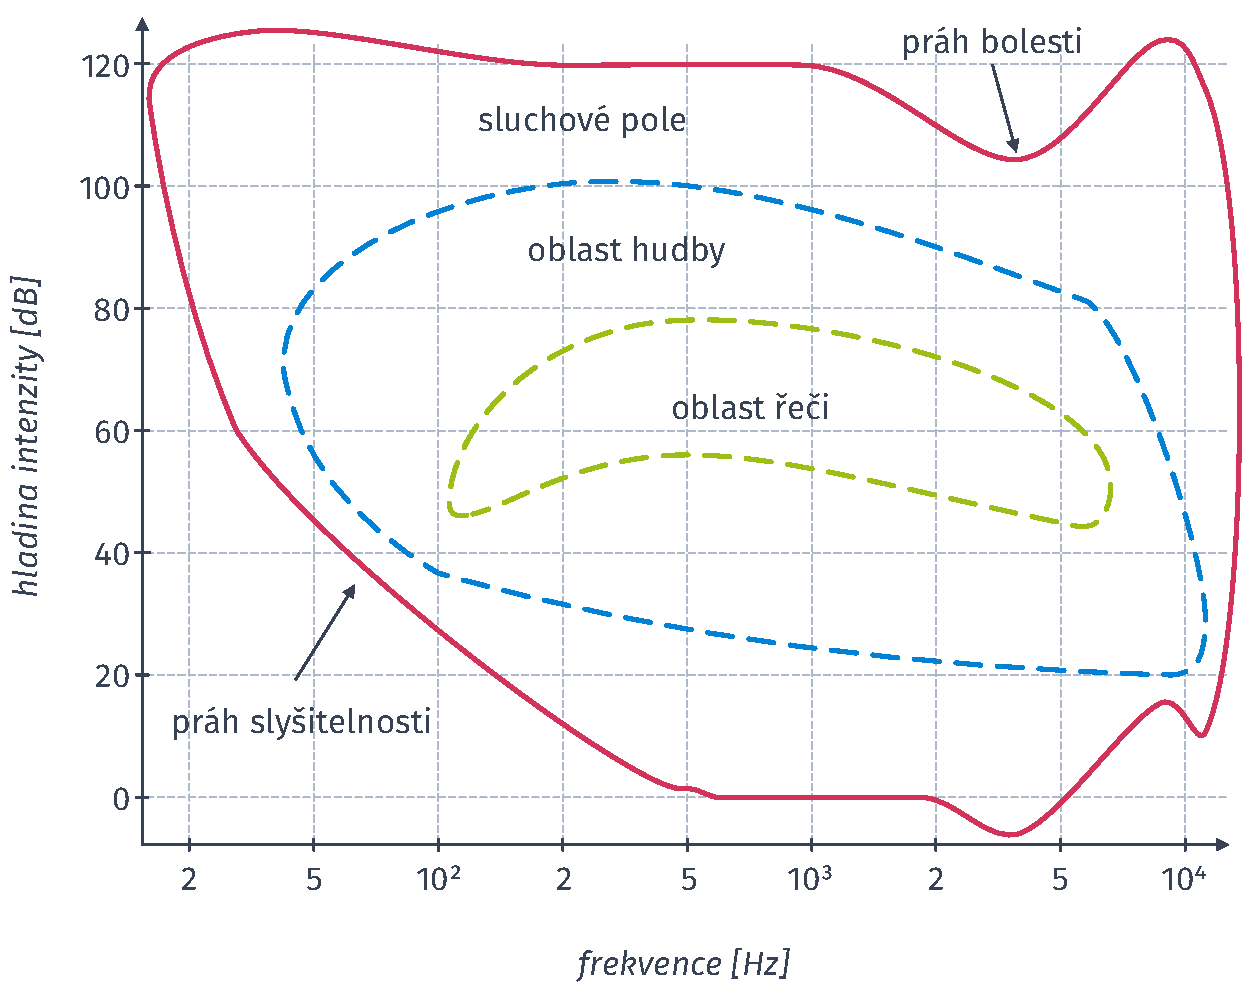
\includegraphics[width=0.75\textwidth]{./ch4-asr/img/listening_perception.pdf}
%   \caption[Charakteristické oblasti vnímání akustického signálu.]{Charakteristické oblasti vnímání akustického signálu lidským sluchem. $L_p = 20log(p/p_0),\ p_0 = 2\cdot10^{-5}\ Pa$.}
%   \label{fig:asr:mfcc:acoustic:characteristic}
% \end{figure}

% Hlasitost zvuku je závislost intenzity na frekvenci a je zcela subjektivní pocit, kterým člověk posuzuje intenzitu daného zvuku. Na obr. \ref{fig:asr:mfcc:acoustic:levels} jsou vyznačeny hladiny hlasitosti, které vznikly spojením bodů ve sluchovém poli (obr. \ref{fig:asr:mfcc:acoustic:characteristic}), odpovídající tónům, které člověk vnímá stejně hlasitě. Z křivek je patrné, že subjektivní hlasitost se mění s~frekvencí zvuku. Zvuky s~nižší frekvencí vnímáme méně hlasitěji než zvuky s~vyšší frekvencí, zejména pak zvuky v~rozmezí $3 - 4\ kHz$ \cite{Psutka2006}.

% \begin{figure}[hbpt]
%   \centering
%   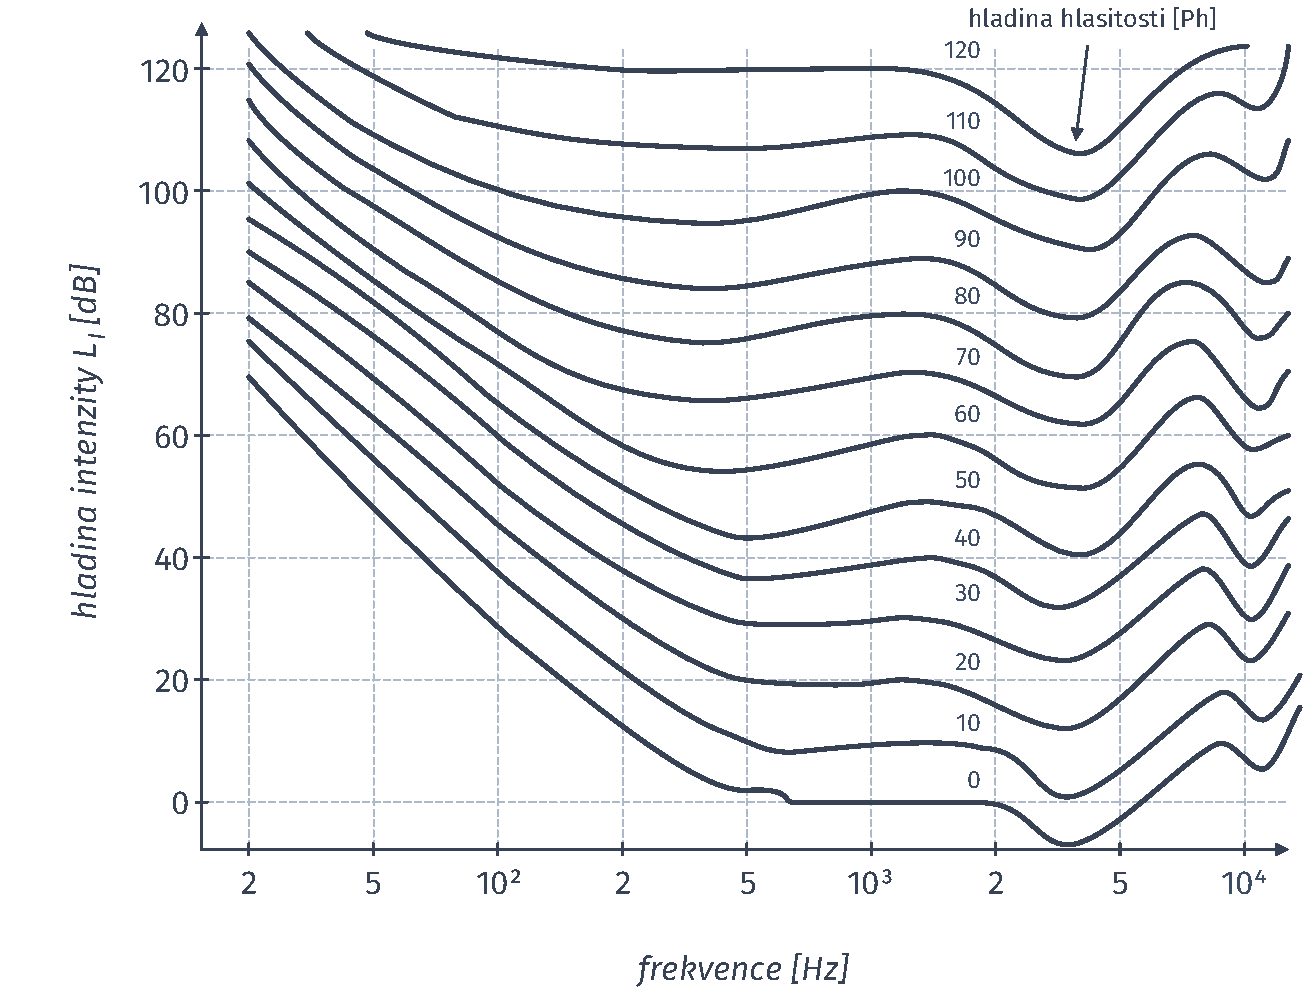
\includegraphics[width=0.75\textwidth]{./ch4-asr/img/listening_levels.pdf}
%   \caption[Křívky stejné hlasitosti.]{Křivky stejné hlasitosti. $L_p = 20log(p/p_0),\ p_0 = 2\cdot10^{-5}\ Pa$.}
%   \label{fig:asr:mfcc:acoustic:levels}
% \end{figure}

% Principem modelování procesu slyšení je postižení kompenzace nelineárního vnímání frekvencí lidským sluchem a respektování maskování zvuků včetně tzv. kritických pásem slyšení. Maskování zvuků je přirozená vlastnost lidského sluchu. Rozumí se jím jev, kdy je vnímání jednoho zvuku ovlivněno přítomností jiného zvuku. Jinými slovy lze říci, že přítomnost jednoho zvuku zvyšuje práh slyšitelnosti pro jiný zvuk. Ten buď zní současně nebo s~drobným časovým odstupem od toho prvního. Tento jev je jakýsi \uv{psychologický filtr}, který ignoruje veškerý šum ležící mimo určité kritické pásmo slyšení. Šířka kritického pásma je přitom závislá na frekvenci poslouchaného tónu.
Často užívanými metodami pro modelování procesu slyšení jsou \textbf{melovská kepstrální filtrace} a \textbf{perceptivní lineární prediktivní analýza}.

% \subsubsection{Melovské kepstrální koeficienty}

% Metoda melovských frekvenčních kepstrálních koeficientů (MFCC) se snaží respektovat výše zmíněné vlastnosti lidského sluchu, především se snaží dodržet kritická pásma slyšení a vliv subjektivního vnímání výšky tónů.

% Základem MFCC je využití banky filtrů a lineárního rozložení frekvencí v~tzv. \textbf{melovské frekvenční škále} definované vztahem

% \begin{equation}
%   f_m = 2595 \log \left(1 + \frac{f}{700}\right),
%   \label{eq:asr:mfcc:melscale}
% \end{equation}

% \noindent kde $f \left[Hz\right]$ je frekvence v~lineární škále a $f_m \left[mel\right]$ je odpovídající frekvence v~melovské stupnici. Melovský filtr má trojúhelníkový tvar. Banka obsahuje $M^{*}$ filtrů rozmístěných lineárně v~melovských frekvenčních souřadnicích, a to tak, že dva sousední filtry se navzájem o polovinu překrývají. Pro střední frekvence jednotlivých filtrů $b_{m,i}$ v~melovské škále platí vztah

% \begin{equation}
%   b_{m,i} = b_{m,i-1} + \Delta_{m},
%   \label{eq:asr:mfcc:freq}
% \end{equation}

% \noindent kde $b_{m, 0} = 0\ mel$, $i = 1, 2,\ \dots\ , M^{*}$, a $\Delta_m = B_{m,w} / (M^{*} + 1)$, kde $B_{m,w}$ je celková šířka pásma v~melovské škále. Ukázka banky filtrů v~této škále je znázorněna na obr.~\ref{fig:asr:mfcc:bank:mel}. Pro výpočet odezvy filtrů je však nezbytné přepočítat všechny koeficienty FFT do melovské frekvenční škály.

% \begin{figure}[hbpt]
%   \centering
%   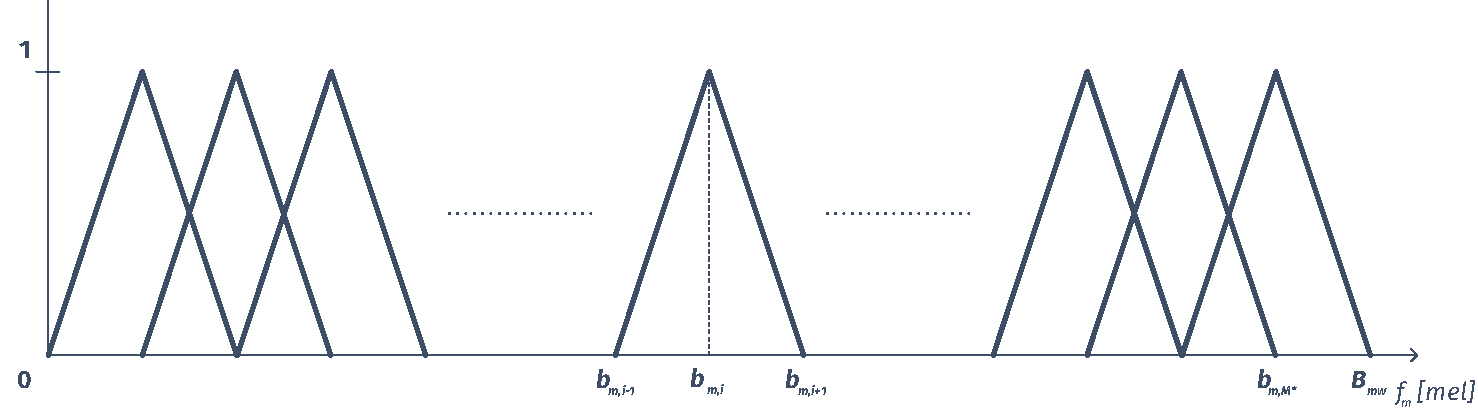
\includegraphics[width=0.9\textwidth]{./ch4-asr/img/filter_bank-mel.pdf}
%   \caption{Rozložení banky trojúhelníkových filtrů v~melovské frekvenční škále.}
%   \label{fig:asr:mfcc:bank:mel}
% \end{figure}

% \noindent Vhodnější je vyjádření trojúhelníkových filtrů ve frekvenční škále s~měřítkem v~herzích. K přepočtu středních frekvencí $b_{m,i}$ se využívá inverzního vztahu  k~(\ref{eq:asr:mfcc:melscale}), tedy

% \begin{equation}
%   f = 700 \left[ \exp\left( 0,887.10^{-3} f_m \right) - 1 \right].
%   \label{eq:asr:mfcc:melscale:inverse}
% \end{equation}

% \noindent Střední frekvence $b_i$ jednotlivých filtrů jsou vyjádřené také v~herzích. Na rozdíl od popisu v~melovské škále jsou filtry rozmístěny nelineárně napříč celým analyzovaným spektrem, viz obr. \ref{fig:asr:mfcc:bank:hz}.

% \begin{figure}[hbpt]
%   \centering
%   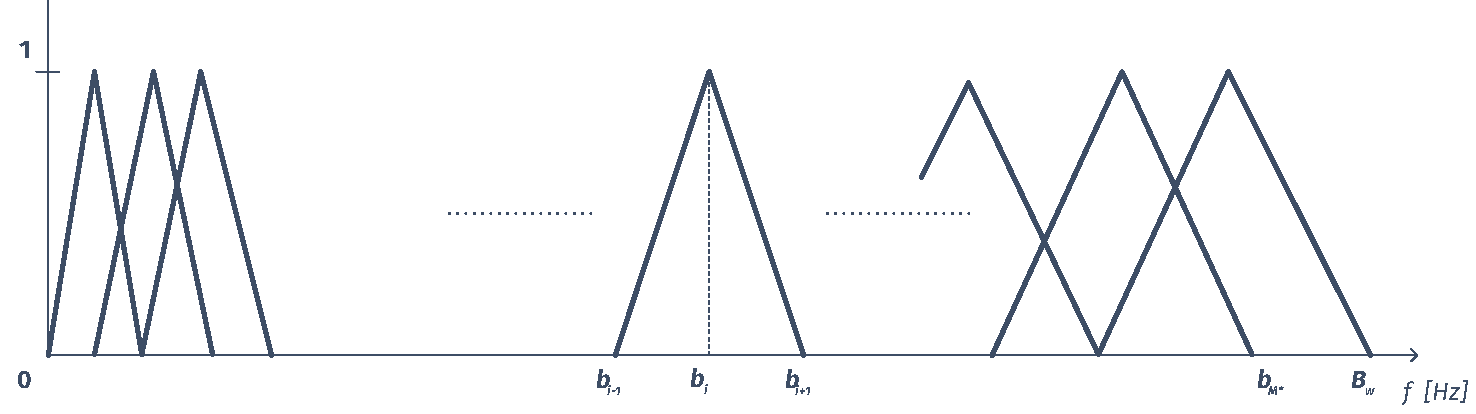
\includegraphics[width=0.9\textwidth]{./ch4-asr/img/filter_bank-hz.pdf}
%   \caption{Rozložení banky trojúhelníkových filtrů ve frekvenční škále.}
%   \label{fig:asr:mfcc:bank:hz}
% \end{figure}

% Na vstup systému jsou postupně přivedeny mikrosegmenty řečového signálu\footnote{Jednotlivé mikrosegmenty byly nejprve předzpracovány, tj. prošly tzv. preemfází. Ta spočívá ve zdůraznění amplitud spektrálních složek řečového signálu s~jejich vzrůstající frekvencí \cite{Psutka2006}.} $s\left(k\right)$ o konstantní délce a pro ně jsou určeny odpovídající koeficienty $c\left(k\right)$. Pro jednotlivé mikrosegmenty je pomocí FFT vypočteno amplitudové spektrum $\left| S(f) \right|$ a následuje klíčová část celého procesu, melovská filtrace. Odezvy filtrů ve frekvenční oblasti lze stanovit pomocí vztahu

% \begin{equation}
%   y_m(i) = \sum_{f=b_{i-1}}^{b_{i+1}} \left| S(f) \right| u\left(f, i\right),  \quad i = 1, 2,\ \dots\ ,M^{*},
%   \label{eq:asr:mfcc:freq:responce}
% \end{equation}

% \noindent kde frekvence $f$ jsou vybírány ze souboru frekvencí využívaných při FFT výpočtu a $u(f, i)$ je vyjádření konkrétního trojúhelníkového filtru $i$. Průchod filtrem tedy znamená, že každý koeficient FFT je násoben odpovídajícím ziskem filtru a výsledky jsou pro příslušné filtry akumulovány. Logaritmováním akumulovaných koeficientů $y_{m}(i)$ je realizován převod do kepstrální oblasti. Tento krok příznivě omezí dynamiku signálu \cite{Benesty2007}. Posledním krokem při výpočtu melovských kepstrálních koeficientů $\left\{c_m\left(j\right)\right\}_{j=1}^{M}$ je provedení IDFT podle vztahu (\ref{eq:asr:lpc:cepstrum:generic}). V~případě MFCC se ale používá diskrétní kosinová transformace (DCT), protože spektrum je reálné a symetrické. K výpočtu slouží vztah

% \begin{equation}
%   c_{m}(j) = \sum_{i=1}^{M^{*}} \log y_m(i) \cos\left( \frac{\pi j}{M^{*}}\left(i - 0,5\right) \right) \quad \text{pro}\ j = 0, 1,\ \dots\ ,M,
%   \label{eq:asr:mfcc:coef}
% \end{equation}

% \noindent kde $M^{*}$ je počet filtrů a $M$ je počet melovských kepstrálních koeficientů. Počet těchto koeficientů $M$ se volí podstatně menší než je počet pásem melovského pásmového filtru $M^{*}$, obvykle se uvažuje prvních $10\ \text{až}\ 13$ koeficientů.

% \subsubsection{Perceptivní lineární prediktivní analýza}

% Stejně jako MFCC, tak také i \textbf{perceptivní lineární prediktivní analýza (PLP)} vychází z lidského vnímání a slyšení zvuků. Snaha je postihnout z psychofyziky slyšení zejména kritická pásma spektrální citlivosti, vztah mezi intenzitou a vnímáním hlasitosti a také křivky stejné hlasitosti \cite{Psutka2006}. PLP podobně jako LPC pak aproximuje získané sluchové spektrum koeficienty autoregresního celopólového modelu.

% Prvním krokem PLP analýzy je \textbf{výpočet výkonového spektra řečového signálu}. Pro konkrétní předzpracovaný\footnote{Ještě před výpočtem je stejně jako u MFCC aplikována preemfáze.} mikrosegment řečového signálu $s(k)$ aplikujeme DFT. Krátkodobé spektrum je pak definováno vztahem

% \begin{equation}
%   P\left(\omega\right) = \left| S\left(\omega\right) \right|^{2} = \left[Re\ S\left(\omega\right)\right]^2 + \left[Im\ S\left( \omega \right) \right]^2.
%   \label{eq:asr:plp:spectr}
% \end{equation}

% \noindent Poté následuje kompenzace nelineárního vnímání změn ve výšce zvuku. Vnímání je logaritmické, proto je nutné provést nelineární transformaci frekvenční osy pomocí vzorce

% \begin{equation}
%   \Omega\left(\omega\right) = 6 \ln \left( \frac{\omega}{1200\pi} + \sqrt{\left(\frac{\omega}{1200\pi}\right)^2 + 1} \right),
%   \label{eq:asr:plp:transform}
% \end{equation}

% \noindent kde $\omega = 2\pi f\ \left[rad/s\right]$ a $\Omega\left(\omega\right)\ \left[Bark\right]$.

% Zahrnutí kritických pásem slyšení (tzv. maskování zvuku) je realizováno navržením vhodného filtru typu pásmová propust šířky jednoho kritického pásma. Stejně jako v~případě MFCC se jedná o banku filtrů, kde na sebe jednotlivé filtry ve frekvenční oblasti navazují.
% Na obr. \ref{fig:asr:plp:filter} je zobrazen průběh jednoho takového filtru. Filtr má strmost $+20\ dB/Bark$ směrem  k~nižším frekvencím a $-50\ dB/Bark$ směrem  k~vyšším frekvencím.

% \begin{figure}[hbpt]
%   \centering
%   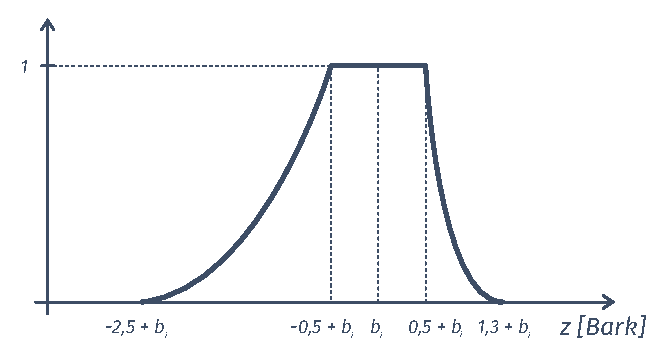
\includegraphics[width=0.5\textwidth]{./ch4-asr/img/plp_filter.pdf}
%   \caption{Ukázka filtru umístěného na Barkově frekvenční ose.}
%   \label{fig:asr:plp:filter}
% \end{figure}

% \newpage \noindent Na Barkově frekvenční ose mají jednotlivé filtry šířku $1$ a jsou podél ní lineárně rozmístěny viz obr. \ref{fig:asr:plp:bank},

% \begin{figure}[hbpt]
%   \centering
%   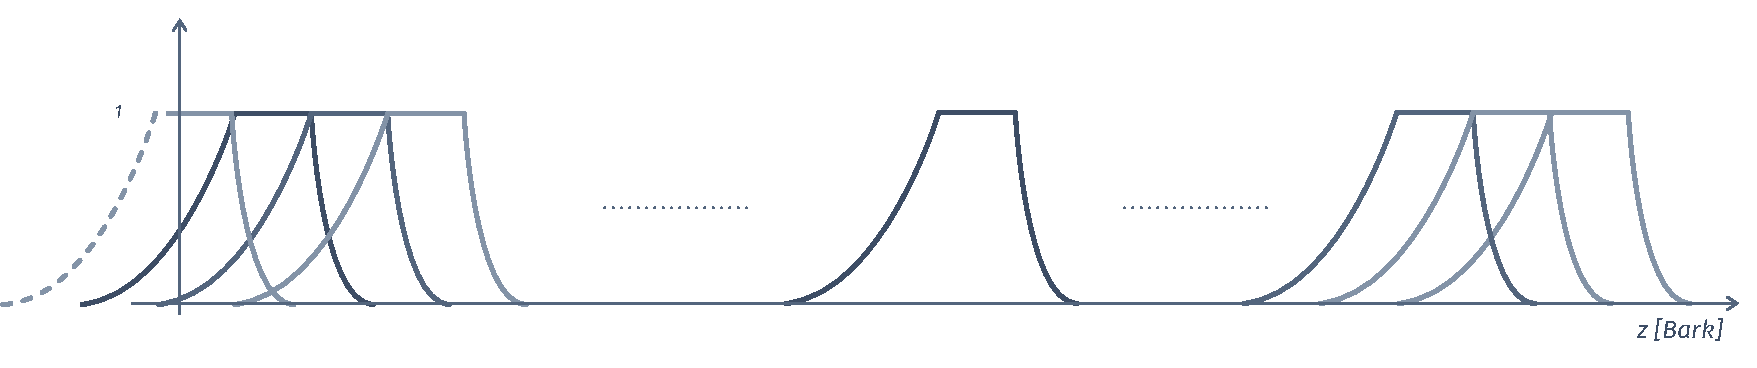
\includegraphics[width=0.9\textwidth]{./ch4-asr/img/plp-bank.pdf}
%   \caption{Rozmístění filtrů na Barkově frekvenční ose.}
%   \label{fig:asr:plp:bank}
% \end{figure}

% Jelikož člověk vnímá intenzitu zvuku v~závislosti na frekvenci nelineárně, tak je potřeba provést \textbf{přizpůsobení křivkám stejné hlasitosti}.
% Na začátku je důležité definovat referenční hlasitost, tj. hlasitost, na kterou bude normalizována.
% Obvykle se volí $40\ Ph$ \cite{Psutka2006}, což přibližně odpovídá hlasitosti běžné řeči. K normalizaci je použit inverzní filtr popsaný vztahem

% \begin{equation}
%   E\left(\omega\right) = K \frac{\omega^4\left(\omega^2 + 56,9 \cdot 10^6\right)}{\left(\omega^2 + 6,3 \cdot 10^6\right)^2\left(\omega^2 + 379,4 \cdot 10^6\right)\left(\omega^6 + 9,6 \cdot 10^{26}\right)},
%   \label{eq:asr:plp:filter}
% \end{equation}

% \noindent kde $\omega = 2\pi f$ a $K$ je konstanta nastavená podle požadovaného zesílení. Přizpůsobení křivce stejné hlasitosti je pak možné například přenásobením celého výkonového spektra mikrosegmentů podle vztahu

% \begin{equation}
%   P'\left(\omega\right) = E\left(\omega\right)P\left(\omega\right),
%   \label{eq:asr:plp:filter:application1}
% \end{equation}

% \noindent kde $P'\left(\omega\right)$ je spektrum transformované na stejnou hlasitost. Případně lze upravit tvar jednotlivých filtrů pomocí vztahu

% \begin{equation}
%   \Phi\left(\omega, i\right) = E\left(\omega\right)\Psi\left(\omega - \omega_i, i\right),
%   \label{eq:asr:plp:filter:application2}
% \end{equation}

% \noindent kde $\Phi\left(\omega, i\right)$ je nový tvar filtru $i$ v~závislosti na frekvenci $\omega$, $\Psi\left(\omega - \omega_i, i\right)$ je odezva filtru $i$ se středovou frekvencí $\omega_i$.

% Po přizpůsobení následuje \textbf{výpočet energie jednotlivých filtrů}, to je obdobné jako u MFCC. Výpočet se provádí pro jednotlivé filtry a výsledky se pak sčítají. Matematicky to je zapsáno vztahem

% \begin{equation}
%   \zeta_m = \sum_{\Omega = \Omega_m - 2,5}^{\Omega_m + 1,3} P\left(\Omega\right)\Phi\left(\Omega, m\right), \quad\ m=1, 2,\ \dots\ M - 2,
%   \label{eq:asr:plp:energy}
% \end{equation}

% \noindent kde $M$ je počet použitých filtrů (kritických pásem).

% Dalším krokem výpočtu je uplatnění \textbf{\uv{zákona slyšení}}. Ten popisuje závislost mezi intenzitou a vnímanou hlasitostí. Na energie $\zeta_m$ je aplikována nelineární transformace vyjádřena vztahem

% \begin{equation}
%   \xi_m = \left(\zeta_m\right)^{0,3}, \quad\ m = 1, 2,\ \dots\ M-2,
%   \label{eq:asr:plp:energy:transform}
% \end{equation}

% \noindent kde $M$ je opět počet filtrů. Díky této operaci dojde také  k~redukci proměnlivosti \uv{výstupů} kritických pásmových filtrů a výsledný hledaný celopólový model může být relativně nízkého řádu.

% Finálním krokem je \textbf{aproximace celopólového modelu}. Ta vychází z výpočtu koeficientů celopólového modelu metody LPC, kde je model popsán vztahem (\ref{eq:asr:lpc:generic:edited}). Pro chybu predikce pak platí

% \begin{equation}
%   e\left(k\right) = \sum_{k} \left(s\left(k\right) + \sum_{i=1}^{Q} a_i s\left(k - i\right)\right).
%   \label{eq:asr:plp:error}
% \end{equation}

% \noindent Aplikací Z-transformace a uvážením rovnice (\ref{eq:asr:lpc:generic}), je možné vztah (\ref{eq:asr:plp:error}) upravit do tvaru

% \begin{equation}
%   E\left(z\right) = \left[1 + \sum_{i=1}^{Q} a_i z^{-i}\right] S\left(z\right) = A\left(z\right)S\left(z\right),
%   \label{eq:asr:plp:error:transform}
% \end{equation}

% \noindent kde $A\left(z\right)$ je model produkce řeči a $E\left(z\right)$, resp. $S\left(z\right)$ jsou získané Z-transformací $e\left(k\right)$, resp. $s\left(k\right)$. Celkovou chybu predikce je pak možné vyjádřit vztahem

% \begin{equation}
%   E\left(z\right) = \frac{1}{2\pi} \int_{-\pi}^{\pi} P\left(\omega\right) A\left(e^{j\omega}\right) A\left(e^{-j\omega}\right)d\omega,
%   \label{eq:asr:plp:error:final}
% \end{equation}

% \noindent kde $P\left(\omega\right)$ je vypočtené výkonové spektrum. Podobně jako u LPC hledané řešení odpovídá hodnotám, pro něž je celková chyba autokorelační funkce $R\left(i\right)$ minimální. Pro konečný počet známých frekvencí je tato funkce definována vztahem

% \begin{equation}
%   R\left(i\right) = \frac{1}{N} \sum_{n=0}^{N-1} P\left(\omega_n\right) \cos\left(i\omega_n\right),
%   \label{eq:asr:plp:error:solution}
% \end{equation}

% \noindent kde $i = 0,\ \dots\ Q$, $Q$ je řád autoregresního modelu a $N$ je počet bodů spektrální charakteristiky. Frekvence $\omega_n$ jsou ty, pro které jsou známé spektrální hodnoty. Pro dobrou aproximaci se volí $Q = 5$ \cite{Benesty2007}. \textbf{Výpočet kepstrálních koeficientů PLP} lze pak pro známé hodnoty $R\left(i\right)$, podobně jako u LPC, určit Durbinovým algoritmem. Nalezené koeficienty lze využít jako příznaky při návrhu parametrizátoru řeči
% \cite{Holmes2001}.

% K vytvoření parametrizátoru je možné použít libovolnou výše popsanou metodu.
% V současnosti ale převládají metody postavené na principu fungování lidského sluchu, protože amplifikují podstatnou informaci zakódovanou v~řeči.
